\section{Kiến trúc tổng thể}\label{sec:architecture}

Hình~\ref{fig:architecture} trình bày kiến trúc tổng thể của hệ thống, lấy nguyên từ sơ đồ kiến trúc của bài báo về CAVAT. Sơ đồ gồm bốn khối: khối dựng gói giáo án từ tài liệu của giáo viên ở phía trên, khối hội thoại dạy học ở giữa, khối chấm điểm và mô hình người học ở dưới khối hội thoại, và quy trình dựng chỉ mục truy xuất ở dưới cùng.

\begin{figure}[ht]
\centering
\makebox[\linewidth]{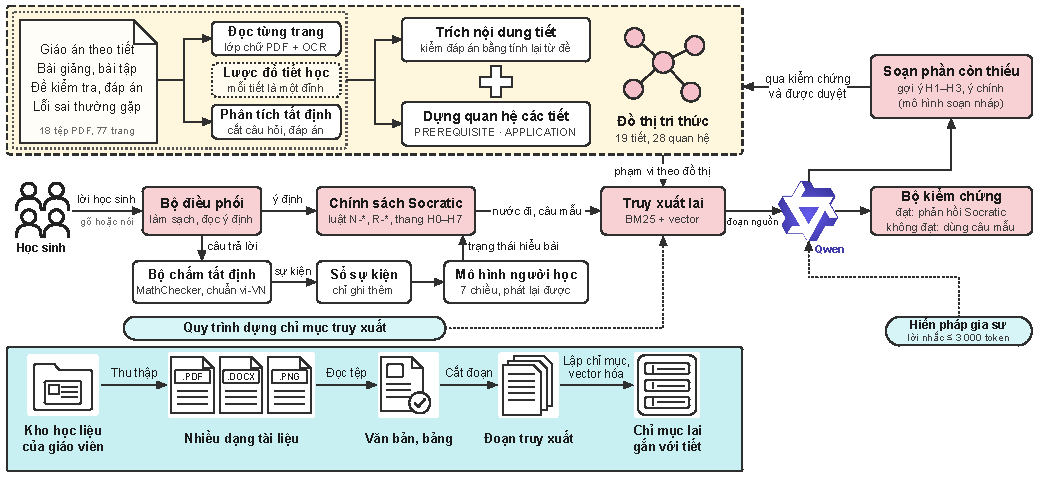
\includegraphics[width=1.1\linewidth]{figures/fig-architecture.pdf}}
\caption{Kiến trúc tổng thể của CAVAT, lấy từ bài báo. Sơ đồ vẽ khi Qwen còn là mô hình duy nhất viết lời; ở bản hiện hành hộp Qwen được thay bằng chuỗi nhiều mô hình do cổng AI điều phối, và Hình~\ref{fig:bandit-flow} bổ sung bộ chọn nước đi bằng bandit vào hộp chính sách Socratic.}
\label{fig:architecture}
\end{figure}

Khối dựng gói giáo án biến tài liệu của giáo viên thành nội dung có cấu trúc mà gia sư dạy được. Hệ thống đọc từng trang của tệp PDF bằng lớp chữ và nhận dạng ký tự, rồi tách thành ba luồng song song: lược đồ tiết học mà mỗi tiết là một đỉnh, phân tích tất định cắt câu hỏi và đáp án, và trích nội dung của từng tiết kèm kiểm đáp án bằng cách tính lại từ đề. Các quan hệ giữa tiết, gồm quan hệ tiên quyết và quan hệ vận dụng, được dựng thành đồ thị tri thức gồm $19$ tiết và $28$ quan hệ. Phần còn thiếu của tài liệu, chẳng hạn gợi ý ở các bậc từ H1 đến H3 hay các ý chính của bài, do mô hình ngôn ngữ soạn nháp, và bản nháp chỉ được dùng sau khi qua kiểm chứng và được giáo viên duyệt.

Khối hội thoại xử lý từng lượt nói của học sinh theo một chuỗi cố định. Bộ điều phối làm sạch lời học sinh và đọc ý định, chính sách Socratic chọn nước đi và mức gợi ý theo luật trên đồ thị và trên từng câu hỏi, và truy xuất lai tìm đoạn nguồn trong phạm vi mà đồ thị cho phép. Mô hình ngôn ngữ nhận nước đi, câu mẫu và đoạn nguồn trong một lời nhắc không quá $3\,000$ token, rồi viết lời gia sư. Bộ kiểm chứng kiểm lời đó: lời đạt thì được gửi cho học sinh, lời không đạt thì được thay bằng câu mẫu đã duyệt.

Khối chấm điểm tách biệt hoàn toàn với mô hình ngôn ngữ. Bộ chấm tất định theo chuẩn viết số của Việt Nam quyết định đúng sai của câu trả lời, mỗi kết quả được ghi thành một sự kiện vào sổ sự kiện chỉ ghi thêm, và mô hình người học bảy chiều tính lại mức hiểu bài từ sổ đó. Trạng thái hiểu bài quay lại làm đầu vào của chính sách để chọn nước đi cho lượt sau. Quy trình dựng chỉ mục ở dưới cùng thu thập kho học liệu của giáo viên gồm nhiều định dạng như PDF, DOCX và ảnh, đọc thành văn bản và bảng, cắt thành đoạn truy xuất, rồi lập chỉ mục và vector hóa để gắn mỗi đoạn với một tiết. Các mục sau của chương mô tả từng thành phần này chi tiết hơn.
